\chapter{Theoretical method}
A protein is thus represented as a point cloud where each of these points
represents an atom of the protein. Aiming at optimizing the time to go through
this point cloud and modelling the interface between both
 proteins, we use the triangulation of Delaunay \cite{Triangulation}.

This triangulation is unique and can be explained like this:
every circumscribed circle of a triangle of the point cloud contains only the
points of the aforementioned triangle (see figure \ref{fig::explication_delaunay}).
We shall explain at first the method to determine the interface in two dimensions(size).

\begin{figure}[ht]
\centering
  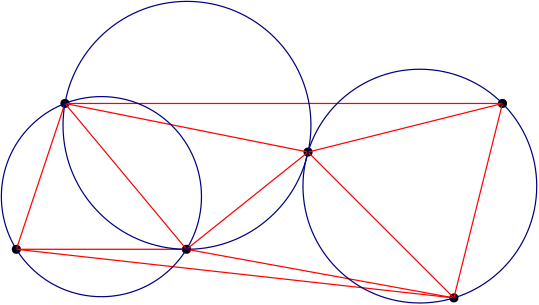
\includegraphics[width=\textwidth]{figures/explication_delaunay.png}
  \caption{Delaunay Triangulation}
  \label{fig::explication_delaunay}
\end{figure}

\section{Dimension 2}

It is necessary to apply this triangulation to the complex of which
 we want to determine the interface, meaning on the coordinates of the atoms that
 form the point cloud (see figure \ref{fig::delaunay_tr}).
  The two proteins of the complex are differentiated by their colors (red and blue)
   on the figure.
   We select then the useful part of this triangulation (see figure \ref{fig::delaunay_reduced}):
    we keep only the triangles which contain at least a point at the interface.

A point is at the interface if it is in a triangle containing at least
a point of every protein. Reducing the size of the triangulation will
be useful afterward to accelerate the processing time and the recovering of the data
concerning the interface.

\begin{figure}[ht]
\centering
\begin{subfigure}{0.4\textwidth}
  \centering
  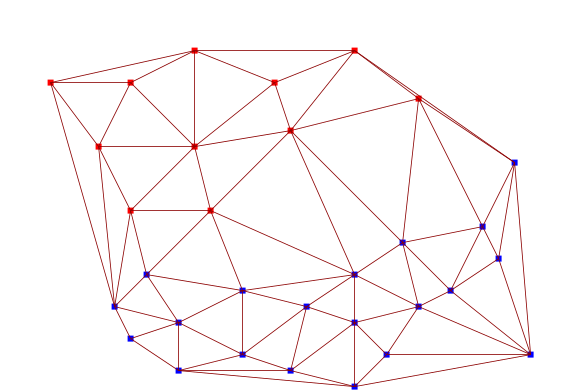
\includegraphics[width=\textwidth]{figures/delaunay.png}
  \caption{Delaunay Triangulation}
  \label{fig::delaunay_tr}
\end{subfigure}%
\begin{subfigure}{0.2\textwidth}
  \centering
  $\Longrightarrow$
\end{subfigure}%
\begin{subfigure}{0.4\textwidth}
  \centering
  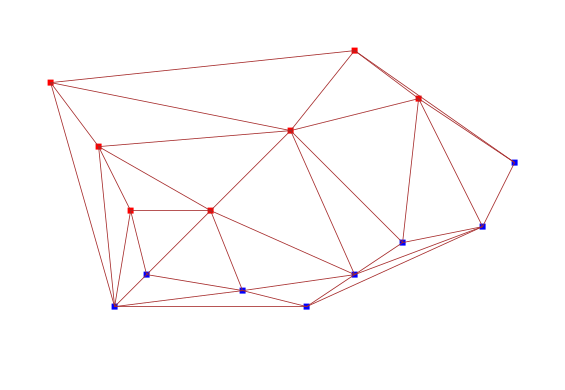
\includegraphics[width=\textwidth]{figures/delaunay_reduced.png}
  \caption{Reduced Triangulation}
  \label{fig::delaunay_reduced}
\end{subfigure}
\caption{Réducing a triangulation}
\label{fig::delaunays}
\end{figure}

We focus now on the determination of the interface itself.
By keeping only the useful edges (see figure \ref{fig::delaunays_process_1}),
 that is those connecting two points belonging to two different proteins,
 we can approximate the interface of contact thanks to the Voronoï diagram.

\begin{figure}[ht]
\centering
\begin{subfigure}{0.45\textwidth}
  \centering
  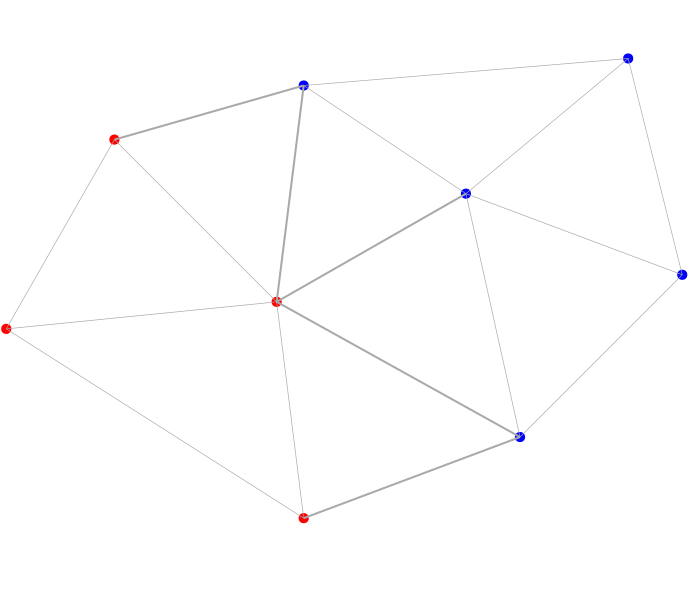
\includegraphics[width=\textwidth]{figures/process_d_1.png}
  \caption{Delaunay Triangulation}
  \label{fig::process_d_1}
\end{subfigure}%
\begin{subfigure}{0.1\textwidth}
  \centering
  $\Longrightarrow$
\end{subfigure}%
\begin{subfigure}{0.45\textwidth}
  \centering
  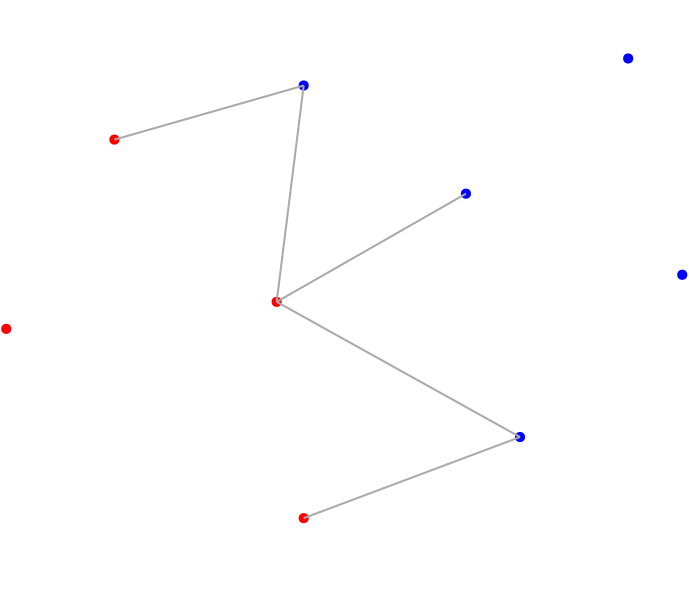
\includegraphics[width=\textwidth]{figures/process_d_2.png}
  \caption{Edges at the interface}
  \label{fig::process_d_2}
\end{subfigure}
\caption{Triangulations et useful area}
\label{fig::delaunays_process_1}
\end{figure}


This diagram is the dual of the Delaunay triangulation and represents points
equally distant from the points of the triangulation (see figure \ref{fig::process_d_3}).
By keeping only the parts of the Voronoï diagram which correspond
 to the previously selected edges (to see figure \ref{fig::process_d_4}),
  we obtain a line strait by pieces which approximates the interface of contact in dimension 2.

\begin{figure}[ht]
\centering
\begin{subfigure}{0.45\textwidth}
  \centering
  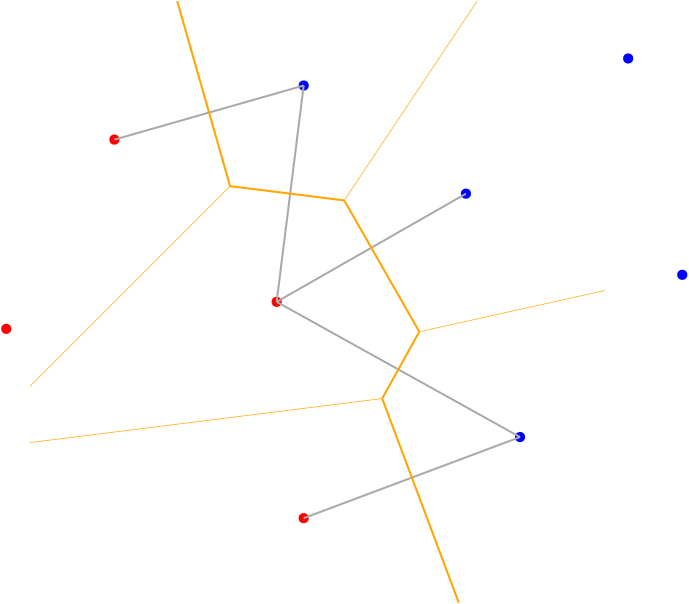
\includegraphics[width=\textwidth]{figures/process_d_3.png}
  \caption{Voronoï Diagramme}
  \label{fig::process_d_3}
\end{subfigure}%
\begin{subfigure}{0.1\textwidth}
  \centering
  $\Longrightarrow$
\end{subfigure}%
\begin{subfigure}{0.45\textwidth}
  \centering
  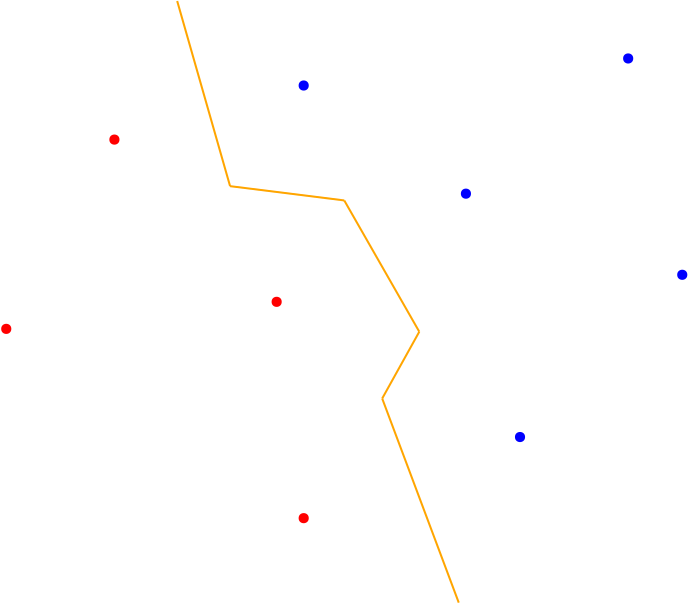
\includegraphics[width=\textwidth]{figures/process_d_4.png}
  \caption{Interface}
  \label{fig::process_d_4}
\end{subfigure}
\caption{Calculation of the surface}
\label{fig::delaunays_process_2}
\end{figure}


\section{Dimension 3}

If we transpose the method seen above in dimension 3, the triangles formed
 by points become tetrahedrons on which we will work to calculate the interface.
  In the same way, a tetrahedron will be considered
at the interface if it contains at least an atom of every protein.
Furthermore, the dual of an edge becomes a surface surrounding this
 edge (see figure \ref{fig::dual_3d}). By gathering
  these pieces, we obtain a surface in three dimensions which models
  the contact area between both proteins of the studied complex.

\begin{figure}[ht]
\centering
  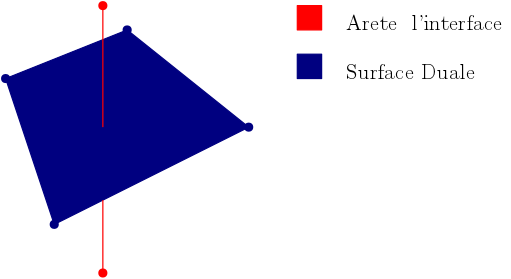
\includegraphics[width=\textwidth]{figures/dual_3d.png}
  \caption{Dual of an edge Dimension 3}
  \label{fig::dual_3d}
\end{figure}

The triangulation in three dimensions of a point cloud corresponding to
 the atoms of a complex gives the figure \ref{fig::delaunays_3d}.

\begin{figure}[ht]
\centering
\begin{subfigure}{0.45\textwidth}
  \centering
  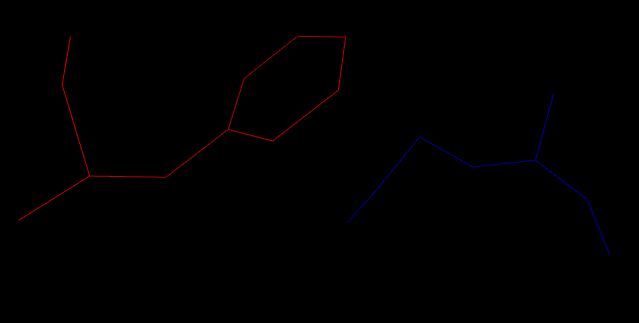
\includegraphics[width=\textwidth]{figures/small_prot.png}
  \caption{Part of a complexe}
  \label{fig::small_prot}
\end{subfigure}%
\begin{subfigure}{0.1\textwidth}
  \centering
  $\Longrightarrow$
\end{subfigure}%
\begin{subfigure}{0.45\textwidth}
  \centering
  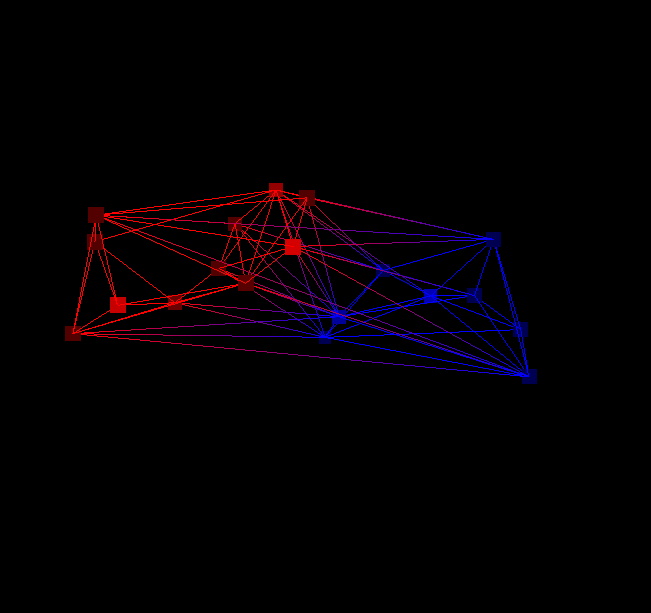
\includegraphics[width=\textwidth]{figures/3d_triangulation04.png}
  \caption{Triangulation}
  \label{fig::prot_delaunay}
\end{subfigure}
\caption{3D Triangulation of a complex}
\label{fig::delaunays_3d}
\end{figure}
